\documentclass{article}
\usepackage{arxiv}
\usepackage[utf8]{inputenc} % allow utf-8 input
\usepackage[T1]{fontenc}    % use 8-bit T1 fonts
\usepackage{hyperref}       % hyperlinks
\usepackage{url}            % simple URL typesetting
\usepackage{booktabs}   
\usepackage{pdfpages}% professional-quality tables
\usepackage{amsfonts}       % blackboard math symbols
\usepackage{nicefrac}       % compact symbols for 1/2, etc.
\usepackage{microtype}      % microtypography
\usepackage{lipsum}
\usepackage{siunitx}
\usepackage[linesnumbered,ruled,vlined]{algorithm2e}
\usepackage{float}
\usepackage{amsmath}
\usepackage{enumerate}
\usepackage{cite}
\usepackage{xcolor}
\usepackage{graphicx}
\graphicspath{ {./images/} }

\newcommand{\note}[1]{\textbf{#1}}

\title{Evolutionary Algorithms}


\author{
 Sherry Usman\\
  4168216\\
  \texttt{s.usman@umail.leidenuniv.nl}\\
  %% examples of more authors
   \And
 Megan Mirnalini Sundaram Rajaraman\\
  4018907\\
  \texttt{m.m.s.rajaraman@umail.leidenuniv.nl} \\
  %% \And
 %% Name \\
  %% Student number\\
  %% \texttt{email address} \\
  %% \AND
  %% Coauthor \\
  %% Affiliation \\
  %% Address \\
  %% \texttt{email} \\
  %% \And
  %% Coauthor \\
  %% Affiliation \\
  %% Address \\
  %% \texttt{email} \\
  %% \And
  %% Coauthor \\
  %% Affiliation \\
  %% Address \\
  %% \texttt{email} \\
}

\begin{document}
\maketitle
 \begin{abstract}
In this paper we explore three main problems (\emph{Low Autocorrelation Binary Sequences Problem}, \emph{N-Queens problem} and \emph{Katsuura problem}) and the various evolutionary strategies that can be used to solve them. For the first two problems, we find a genetic algorithm and a set of hyper-parameters that are optimal for solving both problems. For the \emph{Katsuura} problem,  we find an evolutionary algorithm and experiment with the hyperparameters to find an optimal solution. 
\end{abstract}


% keywords can be removed
%\keywords{First keyword \and Second keyword \and More}


\section{Introduction}\label{sec:intro}
In recent years, metaheuristic algorithms have increasingly become more practical in solving complex real-life in different fields such as logistics and economics, biology.  There are a number of different meta-heuristic algorithms such as single solution algorithms and population-based algorithms. Taking inspiration from real-life biological processes, Evolutionary Algorithms use phenomena like reproduction or recombination, mutation and selection to iterate through a set of candidate solutions to find 'individuals' or solutions with the highest fitness. In this paper we focus on population-based algorithms, especially Evolutionary Strategies and Genetic Algorithms. Like other optimization algorithms, evolutionary algorithms aim to find a solution with the highest fitness and with the highest convergence velocity. 
\section{Methods}
\subsection{Genetic Algorithms}
A subset of evolutionary strategies are genetic algorithms. Genetic algorithms are optimization algorithms that are inspired from Darwin's theory of survival of the fittest and natural selection. A typical GA process involves initializing a random population $P$ of $n$ chromosomes and evaluating the fitness of each chromosome using a fitness criterion or fitness function $F$. Then using fitness-proportional selection methods, a pair chromosomes $C_1$ and $C_2$ are chosen for mating based on their high fitness. The use of a fitness-proportional selection mechanism is an essential part of Genetic Algorithms as it ensures that chromosomes with higher fitness are more likely to be selected than chromosomes with lower fitness and vice versa. Examples of proportional selection methods include roulette wheel where each chromosome is assigned a certain probability proportional to their fitness with the sum of all probabilities being 1. The chromosomes selected during this process are then mated and produce an offspring $O$. Then a crossover mechanism is applied to interpolate between the two parents to generate an offspring. There are many different types of crossover mechanisms, the most common being two-point crossover. Finally, a mutation operation is used to incorporate diversity into the chromosomes produced $O'$.  The new chromosomes are inserted into the population $P$. This process is repeated until an optimum solution is reached or the budget runs out. This algorithm is shown in detail in figure \ref{alg:GA}. As described, genetic algorithms are probabilistic in nature. \\
As seen in the figure, the important parameters that need to be optimized are population size, mutation rate and crossover rate. \\
% In this paper we hope to implement a genetic algorithm that can solve two classical optimization problems: the LABS problem and the NQueens problem. \\ In the following sections we describe both these problems in detail.

\begin{algorithm}[H]
\SetAlgoLined
\SetKwInOut{Input}{Input}
\SetKwInOut{Termination}{Termination}

\Input{Population size $N$, Crossover probability $p_c$, Mutation probability $p_m$, Number of generations or budget $B$}
\Termination{The algorithm terminates when the maximum number of generations $B$ is reached or a stopping criterion is met.}
\BlankLine
Initialize population $P$\;
Evaluate the fitness of the population $F(P)$\;
\While{$t < B$ \textbf{and} stopping criterion not met}{
    $P'(t) \leftarrow \text{MatingSelection}(P)$\;
    $P''(t) \leftarrow \text{Crossover}(P'(t), p_c)$\;
    $P'''(t) \leftarrow \text{Mutation}(P''(t), p_m)$\;
    Evaluate the fitness of $P'''(t)$\;
    Update population: $P \leftarrow P'''(t)$\;
}
\caption{Genetic Algorithm}\label{alg:GA}
\end{algorithm}
For solving the LABS and N-Queens problem,  n-point crossover is taken as the choice of crossover. 
\subsection{Evolutionary Strategies}
Another subset of evolutionary algorithms is Evolutionary Strategies. Evolutionary strategies are a class of metaheuristic algorithms that mimic the adaptive processes in biological evolution and in the real world. The idea of mimicking evolution for optimization was first borne in Germany, which was later developed by Ingo Rechenberg \cite{source_evo1} and Hans-Paul Schwefel \cite{source-evo2}. One of the key differences is that Evolutionary Strategies focus on real-valued search space $\mathbb{R}^n$. The selection is also deterministic in nature (the selection is between $(\mu, \lambda)$ or  $(\mu + \lambda)$. Another key difference is that evolutionary strategies emphasize on mutation. \\
The below mentioned algorithm \ref{alg:ES} shows a generalized ES model. \\
\begin{algorithm}[H]
\SetAlgoLined
\SetKwInOut{Input}{Input}
\SetKwInOut{Termination}{Termination}
\Input{Population $P$, Number of generations or budget $B$} %, Crossover probability $p_c$, Mutation probability $p_m$,% 
\Termination{The algorithm terminates when the budget $B$ is met}
\BlankLine
 t $\rightarrow 0 $ ;\\
Initialize population $P$\;
Evaluate the fitness of the population $P(t)$\;
\While{$t < B$}{
    $P'(t) \leftarrow \text{Recombine}(P (t), p_c)$\;
    $P''(t) \leftarrow \text{Mutate}(P'(t), p_m)$\;
    $P'''(t) \leftarrow \text{Select}(P''(t) \cup Q)$\; 
    Evaluate the fitness of $P'''(t)$\;
    Update population: $P (t+1) \leftarrow P'''(t)$\;
    Update budget $t \leftarrow t + 1$\;
}
\caption{Generational Evolutionary Strategy Model}\label{alg:ES}
\end{algorithm}

Unlike genetic algorithms which focus on schema processing, evolutionary strategies focus on convergence speed and are self-adaptive in mutation. The mutation here, is controlled by a scaling variable $\sigma$. $\sigma$ can be a single step size for all the values in the popultation, or can be adapted or scaled with respect to each of the values.  This is taken from the behavior of repair enzymes, mutator-genes, which increase with respect to the frequency, and this is done to maximise the progress and adapt the shape of the mutation to the local topology. \cite{hao-paper-evostrat} \\
% For this problem, a self-adaptive ES is taken with the scaling factor given below. 
% \begin{equation*}
%  f (x) = \sum_{i=1}^{n} i x_i^2     
% \end{equation*}
For solving the Katsuura optimization problem, a mutation with normal noise added to it, has been implemented and intermediate recombination has been taken as the method of recombination. Intermediate recombination is done by taking the arithmetic mean of both parents, and is varied by the position taken.

\section{Problem}
Algorithm \ref{alg:GA} is used to solve the LABS problem (Section \ref{sec:labs}) and the N-Queens Problem (Section \ref{sec:nqueens}), while algorithm \ref{alg:ES} is used to solve the Katsuura problem. 
\subsection{Low Auto-Correlation Binary Sequences}\label{sec:labs}
Binary sequences are used in a variety of fields such as in radar applications, telecommunication and cryptography. \\
Low Auto-correlation Binary Sequences (LABS) problem is a problem to find a sequence $S = (s_1, s_2 ... s_N)$ with $ s_i = +-1$ such that the energy of the autocorrelation of the sequence is minimum or equivalently, the merit factor is maximum.  The autocorrelation of a sequence S is defined as 
\begin{equation*}
    C_k(S) = \sum_{i=1}^{N-k}s_is_{i+k}
\end{equation*}
for $k  = \{0,..,N-1\}$. The energy of the autocorrelation is defined by the equation: 

\begin{equation*}
    E(S) = \sum_{k=1}^{N-1}C_k^2(S)
\end{equation*}
Low Autocorrelation Binary Sequences (or LABS) are vital in the fields of  synchronization, active sensing systems, cryptography and radar application and communications engineering \cite{9422706}. An important example is in the field of telecommunication where sequences with low auto-correlation are used as modulation pulses in radar and sonar ranging. It is also used in applications such as measurement of space-time curvature. \cite{Packebusch_2016}.\\
Finding the LABS is a difficult computational and optimization problem. The exact solutions for the highest merit factors have been found and documented here \cite{Ukil_2010}. But as the evaluation increases, it exceeds the minimum energy level and that is why it is a complex optimization problem.\\

\subsection{N Queens Problem}\label{sec:nqueens}
The N-Queens problem is a classical optimization problem. This is a generalized formalization of the 8-Queens problem, which was proposed by the chess player Max Bezzel in 1848. The goal is to place $n$ queens in an $n \cdot n$ chessboard such that none of the queens attack each other. In any classical chess game, a queen can move horizontally, diagonally and vertically. \\ 
The constraints of the N-Queens problem are mentioned below.  \cite{n_queens}
\begin{itemize}
    \item Each row should have exactly one Queen. 
    \item Each column should have exactly one Queen.
    \item No two queens should be in the same diagonal.
\end{itemize}
N-Queens Problem, along with LABS belong to PBO problem suite, which is defined as a set of 25 problems of  \textit{Pseudo-Boolean Optimization} nature \cite{IOHprofiler}. 

\subsection{Katsuura Optimization Problem} \label{sec:katsuura}
Katsuura global optimization problem is a multi-modal minimization problem. It can be represented as \cite{katsuura-source}
\begin{equation*}
     f_{Katsuura}(n, x) = \frac{10}{D^2} \prod_{i=0}^{D} \left ( 1 + i \sum_{j=1}^{32} \frac{|2^jz_i- |2^j z_i||}{2^j} \right )^{10/D^{1.2}}-\frac{10}{D^2} + f_{pen}(x) + f_{opt}
\end{equation*}
This complex function forms one of the benchmarks of optimization. This function is part of the functions which were proposed by Hidefumi Katsuura \cite{katsuura-actualpaper}. It is described as \textit{continuous everywhere and differentiable nowhere} which means that this function is continuous, but has no well-defined slope, looking "rugged" \cite{rugged-boi}. This contributes to multiple local minima, thus making it a great problem for optimization and minimization. \\
Katsuura is one of the problems in the BBOB  (\textit{Black Box Bayesian Optimization Benchmarking Suite}) test suite.

\section{Experiments} \label{sec:exp-results}
We want to find a set of evolutionary algorithms that can find the solution to both the N-Queens problem and the LABS problem using the same set of hyperparameters and optimization techniques. Due to the nature of these two problems we decide to go with genetic algorithms, with a solution similar to the one discussed in \ref{alg:GA}. Similarly, for solving the Katsuura Optimization algorithm, a solution similar to the one discussed in \ref{alg:ES} was implemented.   \\
The experiment was performed using \textit{IOHExperimenter}. \cite{IOHexperimenter}
\subsection{Hyper-parameter tuning}
For all three problems, a set of hyperparameters for population size, mutation rate and crossover rate have been explored to arrive at the optimal solution. A table discussing the settings has been given in Table \ref{tab:hyperparameter-tuning}. 
\begin{table}[h!]
    \centering
    \begin{tabular}{|c|c|} \hline 
        \textbf{Hyperparameters} & \textbf{Values}  \\ \hline
        \textbf{Population Size} & \{50, 100, 200, 1000\}  \\ \hline
        \textbf{Mutation Rate}   & \{0.01, 0.1, 0.5\} \\ \hline  
        \textbf{Crossover Rate}  & \{0.5, 0.7, 0.9\} \\ \hline
    \end{tabular}
    \caption{Hyperparameters for tuning the three problems}
    \label{tab:hyperparameter-tuning}
\end{table}

\subsubsection{Population Size}
The population size determines the number of individuals in the initial population and also determines the number of individuals retained in each subsequent generation of the population. The size of population is an important consideration in a genetic algorithm as it prevents 

\subsubsection{Crossover Rate}
Crossover rate determines the number of crossover points selected in two parents.

\subsubsection{Mutation Rate}
Mutation rate in a population determines the rate at which bits in the offspring are flipped to generate new candidate solutions. This parameter controls the rate of diversity of new offspring candidate solutions generated from a set of parents.  

% \begin{algorithm}[!ht]
% \SetAlgoLined
% \SetKwInOut{Input}{Input}\SetKwInOut{Termination}{Termination}

% \Input{Alg.~\ref{alg:ES}, a tuning budget $B$, and objective functions }
% \Termination{The algorithm terminates when..}
% \BlankLine

% \caption{Tuning procedure}\label{al:tuning}
% \end{algorithm}


\section{Results}\label{sec:results}
The results were graphed using IOHAnalyzer \cite{IOHanalyzer} for the expected running time of each hyperparameter setting, 

% Description of the experiments and the results. Use the tables and figures generated from the IOHanalyzer. Make sure to present your results in a way that is convenient to the reader. \textbf{do not blindly include plots of all your experiments; try to combine information in figures and tables!} 

% Figure \ref{fig:example} and \ref{fig:test} show examples of how to insert your figure in the report. Please also see the captions. Make sure you explain your figures properly in the captions.

% \begin{figure}[h!]
%  \begin{center}
%  \includegraphics[width=0.95\textwidth]{example.png}
%  \end{center}
%  \caption{By $n\ln(n)$ normalized average optimization times for OneMax, for $n$ between 500 and 10 000. Displayed numbers are for $n = 10 000$ \cite{ye2019interpolating}.}
%  \label{fig:example}
% \end{figure}


% \begin{figure}[h!]
%  \begin{center}
%  \includegraphics[width=0.95\textwidth]{best-so-far.png}
%  \end{center}
%  \caption{The fixed-target results of 11 algorithms. The figure is downloaded from IOHanalyzer.}
%  \label{fig:test}
% \end{figure}
\subsection{LABS}
The figure \ref{fig:ert-labs}
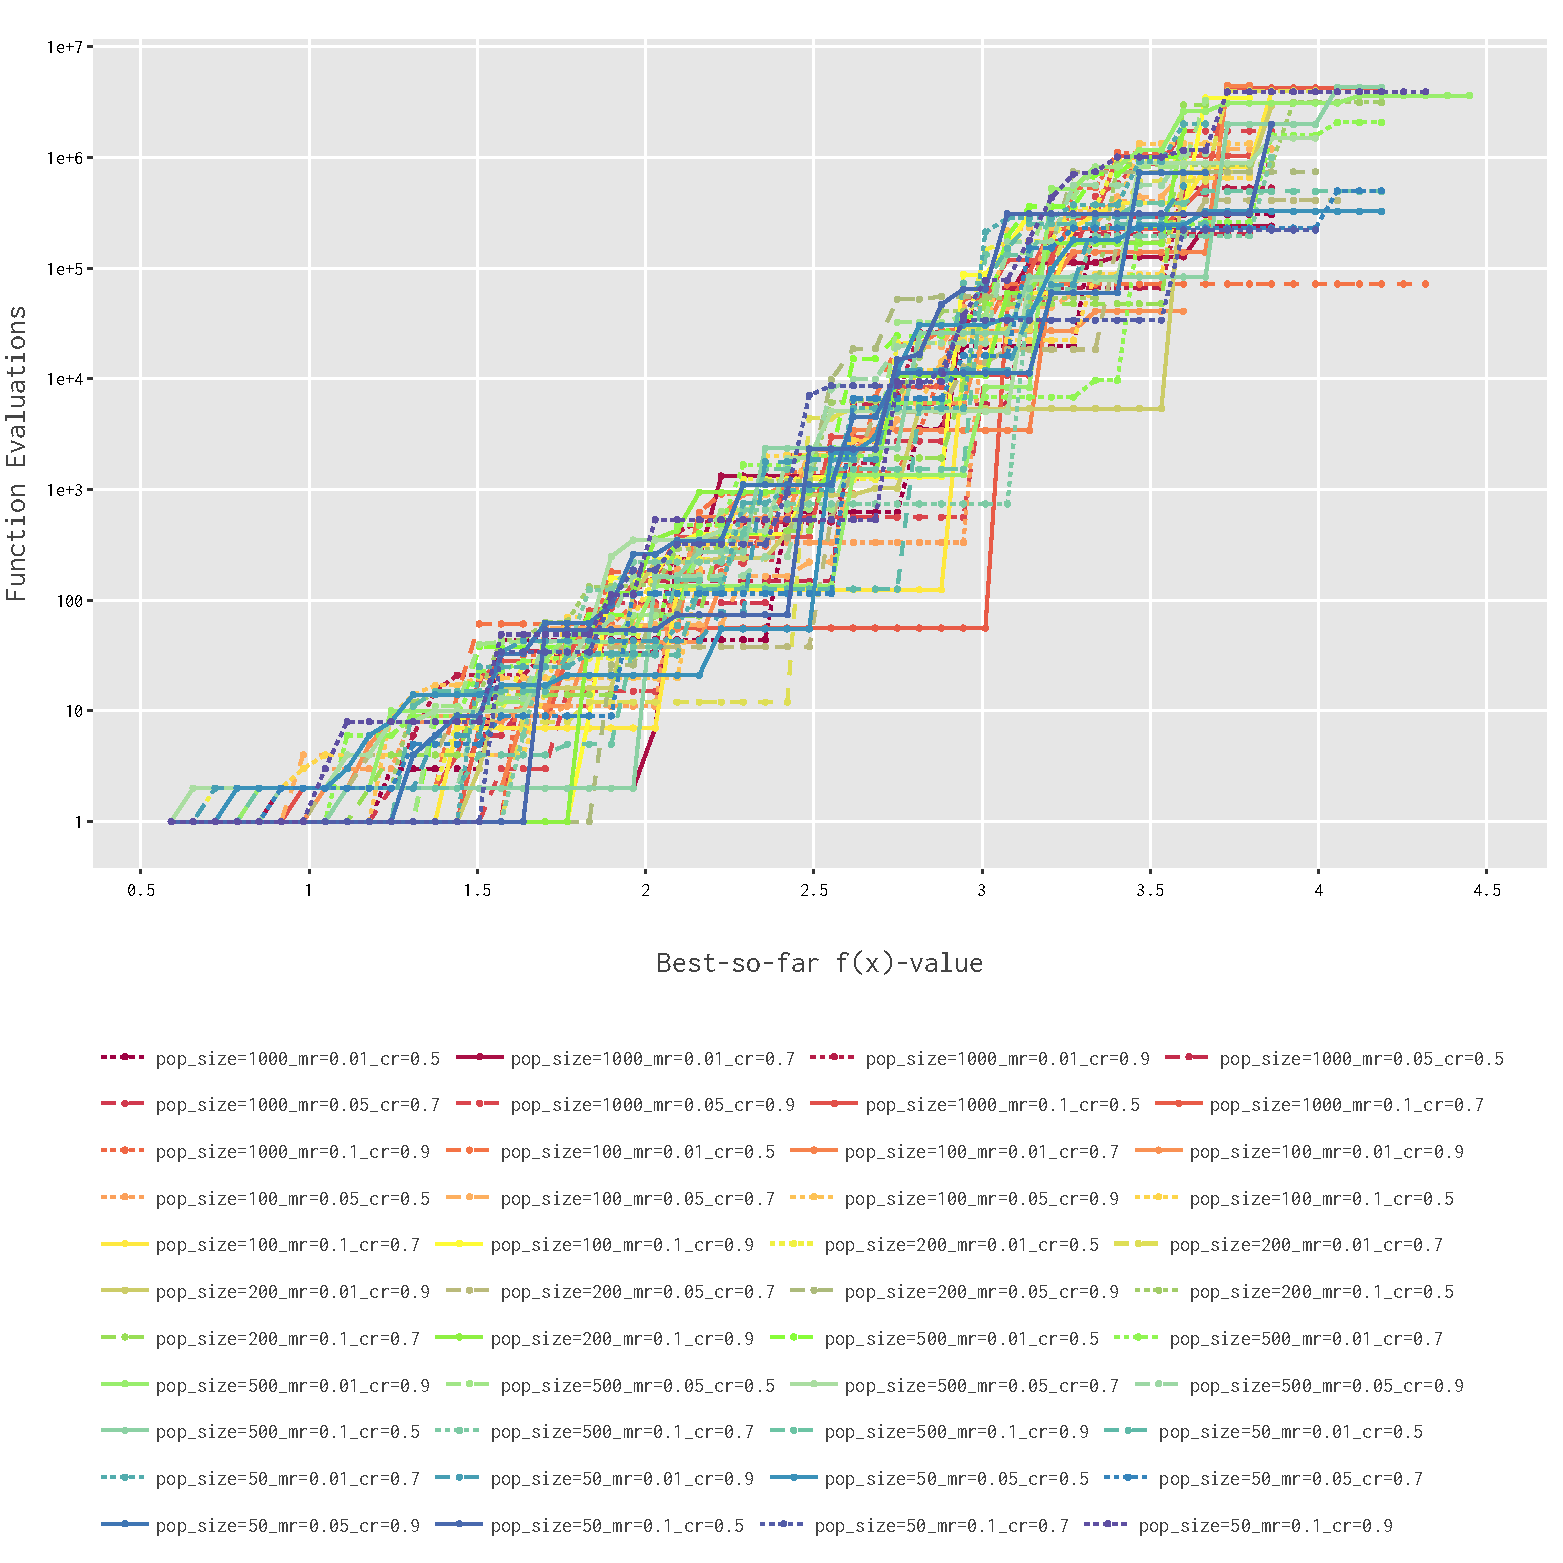
\includepdf[pages=-]{ERT-f18.pdf}\label{fig:ert-labs}

\subsection{N-Queens}
\label{app:f23-runningtime}
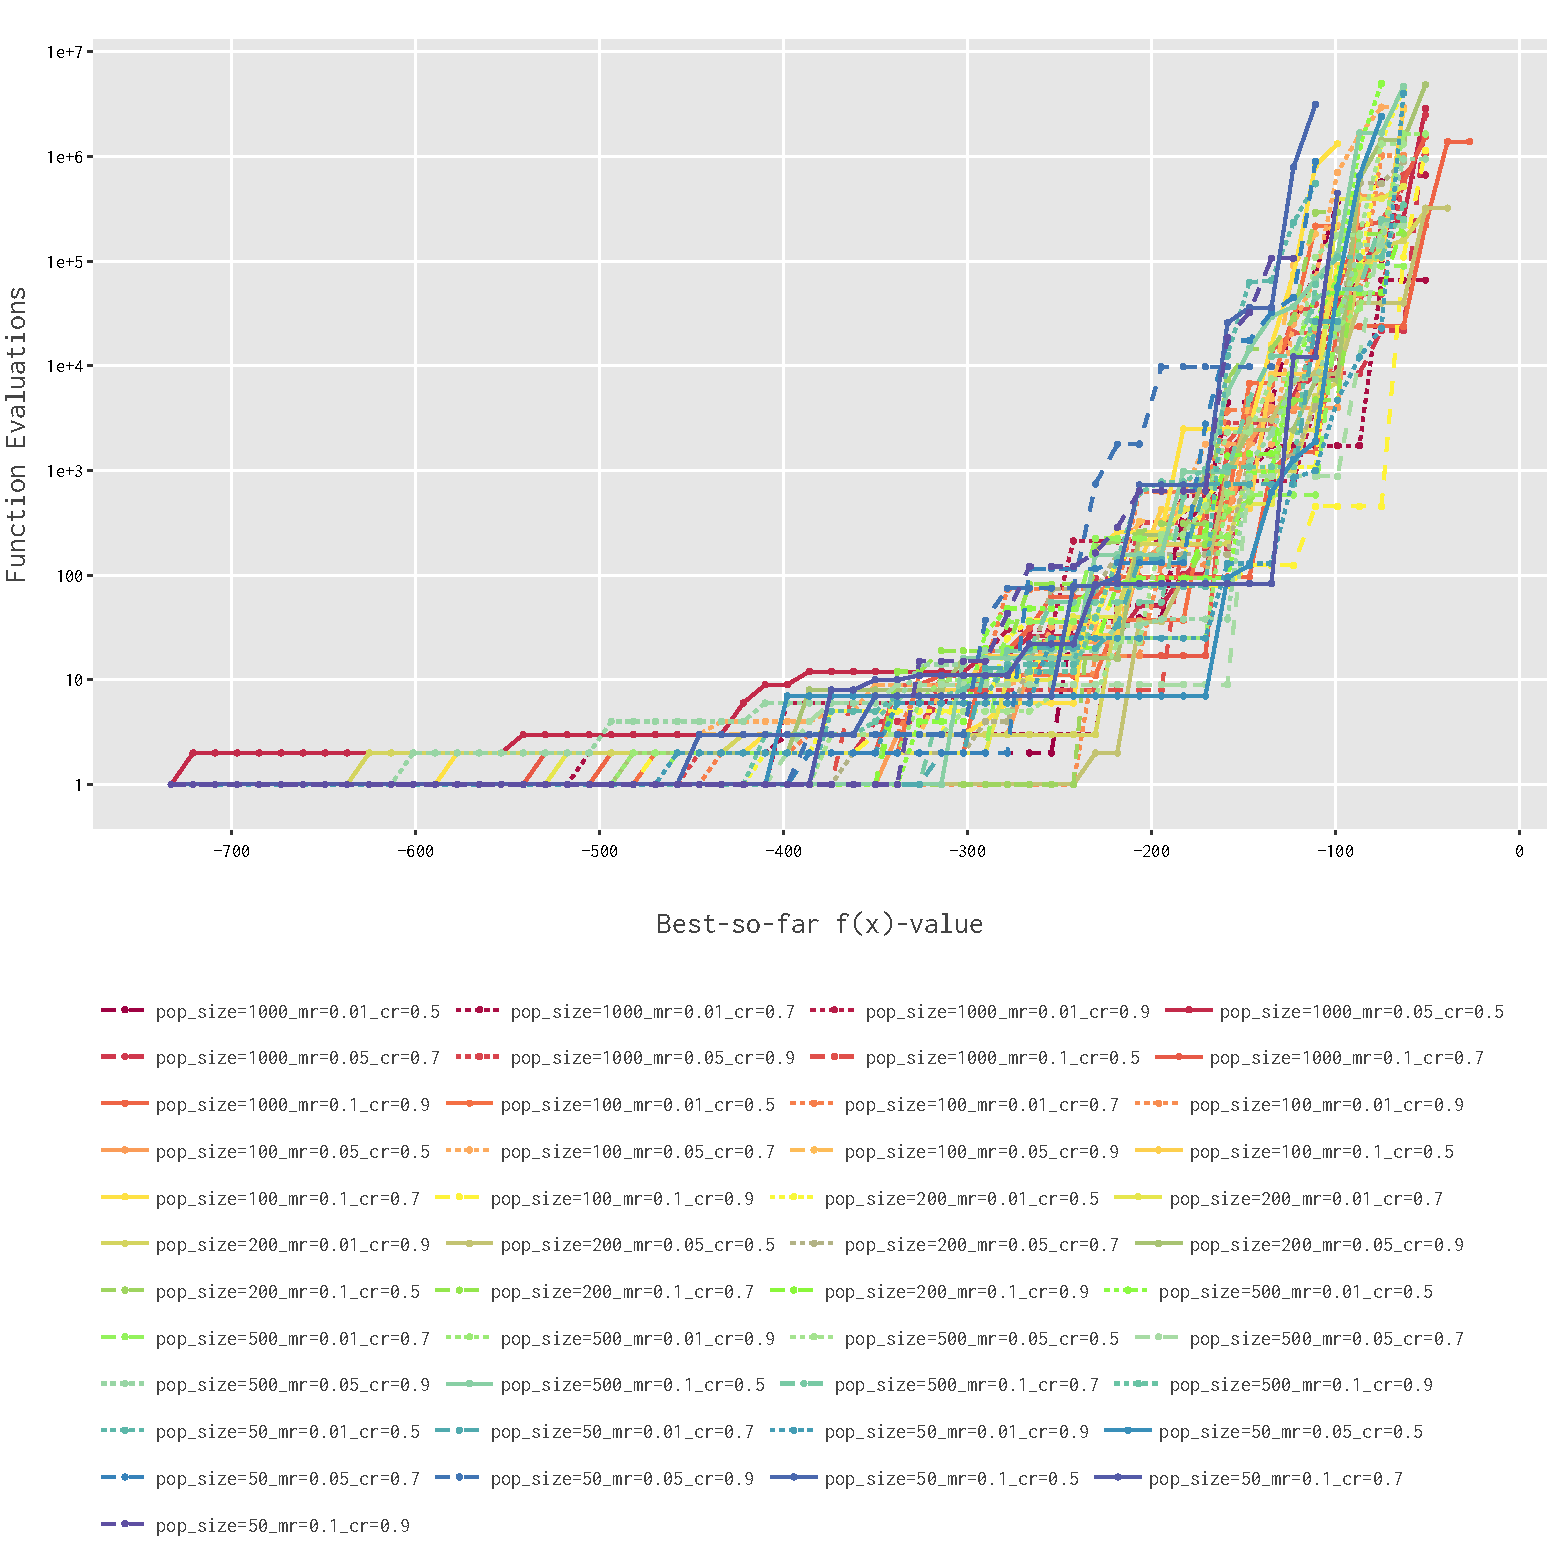
\includepdf[pages=-]{ERT-f23.pdf}\label{fig:ert-nqueens}

\subsection{Katsuura Problem}
The results of the runs were examined and the results were graphed in  Figures\ref{fig:cumulative_distribution-Katsuura} - \ref{fig:shapley-katsuura}. Based on the experiments, the optimal hyperparameter settings were found to be \texttt{mutation\_rate = 0.01, crossover\_rate = 0.9 and population\_size = 20}.\\
Figures \ref{fig:cumulative_distribution-Katsuura} and \ref{fig:emp_cumulative_distribution-Katsuura} refer to the Cumulative Distributions of the problem, with multiple hyperparameter sets. The function evaluations are taken against the proportion of runs for convergence, which shows the ECDF curves for each function setting. As seen from the figure, the optimal setting shows the maximal function value quicker. This is also seen in \ref{fig:emp_cumulative_distribution-Katsuura}
 \begin{figure}[h!]
    \centering
    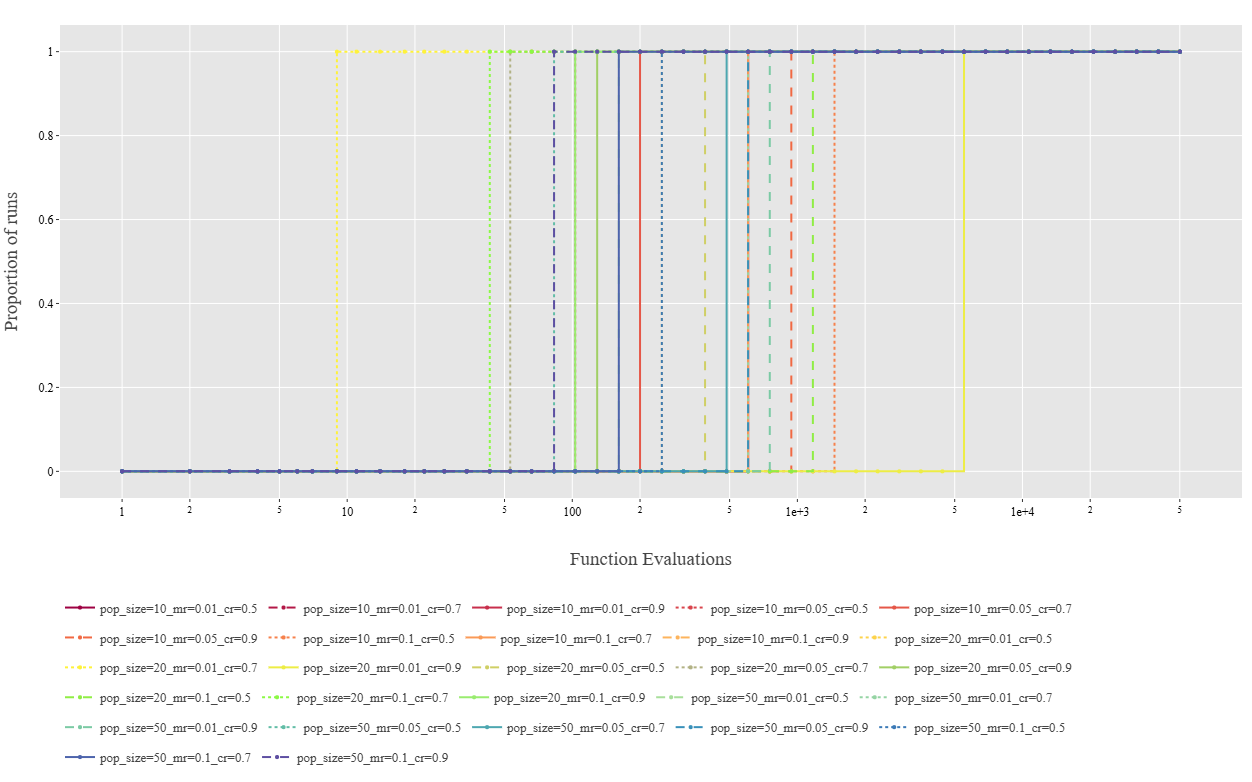
\includegraphics[width=1\linewidth]{Graphs/Katsuura/Cumulative_Distribution.png}
    \caption{ECDF Curves for various hyperparameter settings of the Katsuura Optimization function. The x-axis refers to the function evaluations, and the y-axis refers to the proportion of runs. Out of all the curves, the optimal settings seem to converge the quickest, with the highest maximal function value of all. }
    \label{fig:cumulative_distribution-Katsuura}
\end{figure}

\begin{figure}[h!]
    \centering
    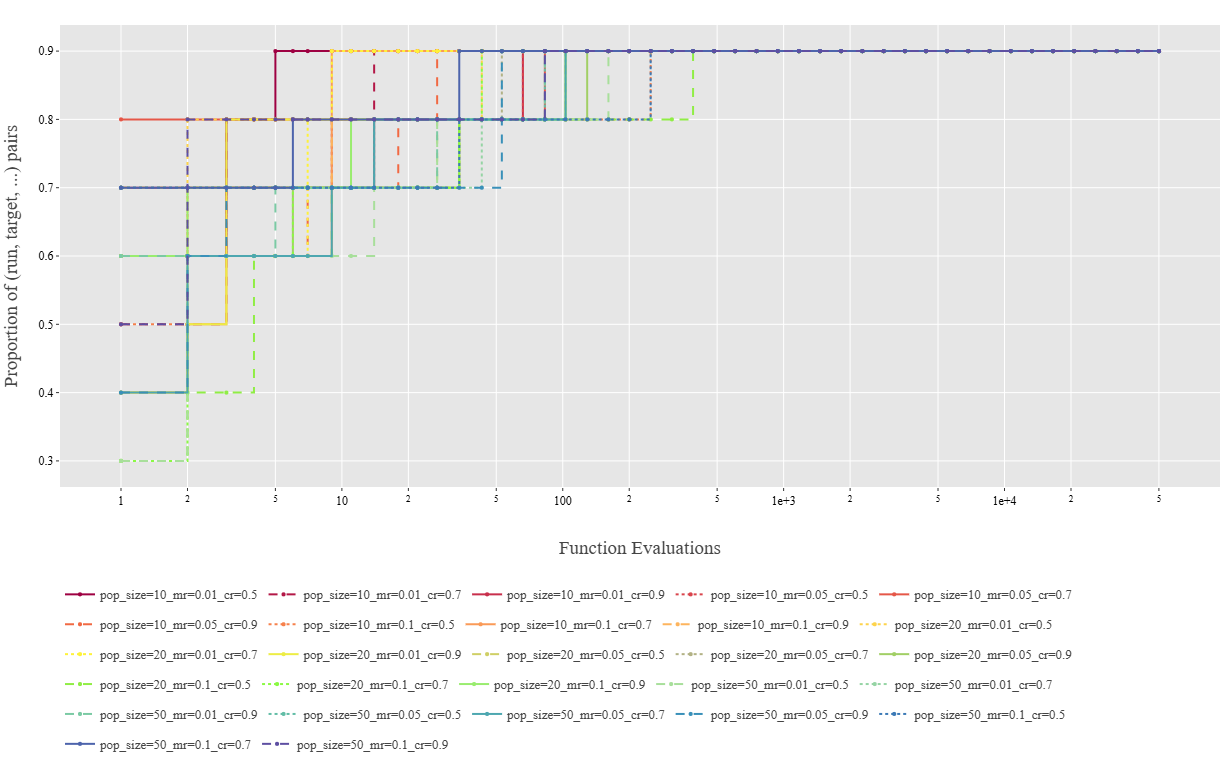
\includegraphics[width=1\linewidth]{Graphs/Katsuura/Empirical_Cumulative_Distribution.png}
    \caption{ECDF Curves for various hyperparameter settings of the Katsuura Optimization function. The x-axis refers to the function evaluations, and the y-axis refers to the proportion of runs and targets evaluated in pairs. }
    \label{fig:emp_cumulative_distribution-Katsuura}
\end{figure}
The next evaluation metric is the best fitness value and the expected runtime for the corresponding value. This is shown in Figures \ref{fig:ert-single-Katsuura} and \ref{fig:ert-multiple-Katsuura}, where the expected runtime is taken for a single and multiple functions respectively. For  figure\ref{fig:ert-multiple-Katsuura}, the mean of the running time samples is taken for evaluations. Although it is not clear in the beginning which function performs well, as the budget is depleted, it becomes clear that the optimal setting converges faster, and has a faster ERT than others. 
\begin{figure}[h!]
    \centering
    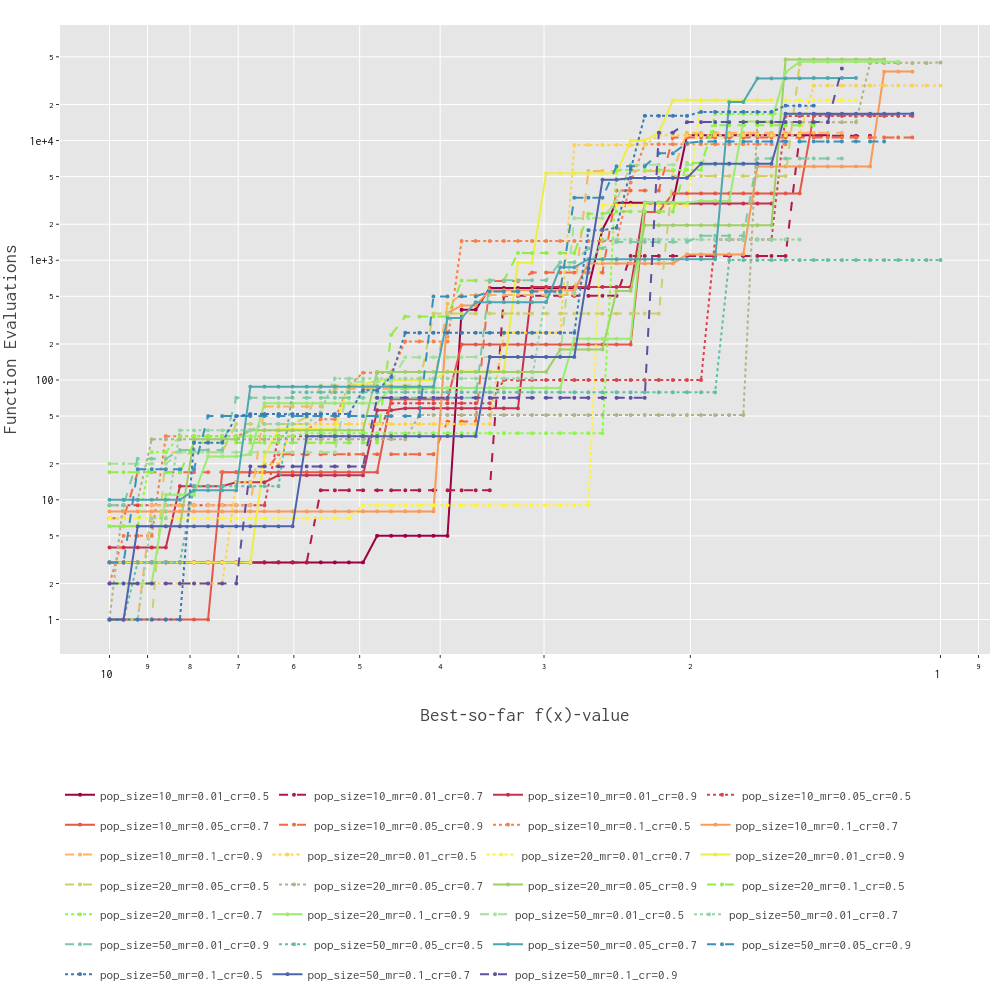
\includegraphics[width=1\linewidth]{Graphs/Katsuura/Expected_RunTime.png}
    \caption{Best value of the function against the budget for the evaluations. The x-axis refers to the function value, and the y-axis refers to the function evaluations (budget) of the problem. The optimal setting, while taking a lower fitness value in the beginning, outperforms others at the end of the given budget. }
    \label{fig:ert-single-Katsuura}
\end{figure}
\begin{figure}[h!]
    \centering
    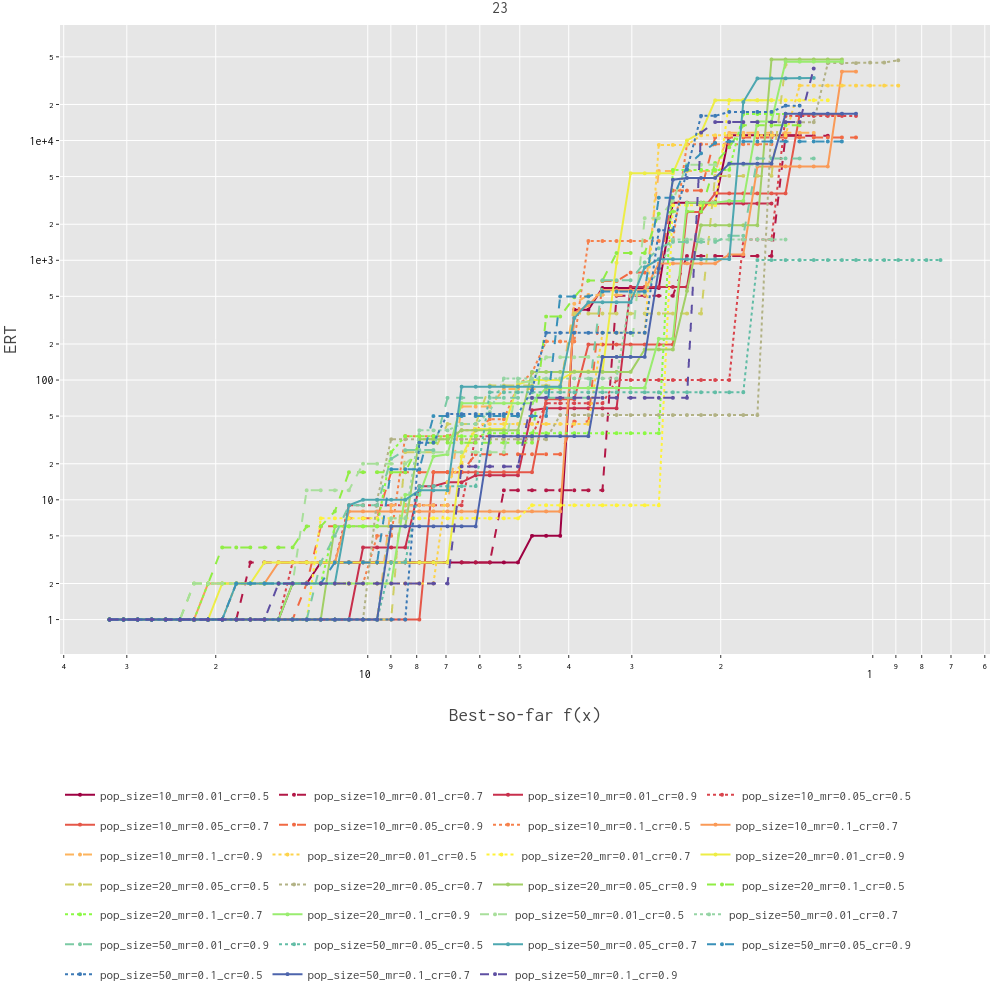
\includegraphics[width=1\linewidth]{Graphs/Katsuura/Expected_RunTime_Multi.png}
    \caption{Best value of the function against the expected run time (ERT) for the hyperparameter setting. The x-axis refers to the function value, and the y-axis refers to the ERT of said function. Here, it is evident that the optimal setting, while taking a lower fitness value in the beginning, outperforms others and converges faster (also seen in figure \ref{fig:ert-single-Katsuura}). }
    \label{fig:ert-multiple-Katsuura}
\end{figure}

In addition to the expected runtime and ECDF curves, the ranking of the functions as well as the contributions of each function are plotted in \ref{fig:ranking-Katsuura} and \ref{fig:shapley-katsuura}. Figure \ref{fig:ranking-Katsuura} shows the ranking of the hyperparameter settings under a fixed-target setting. It is established that the optimal setting is the best, followed by four other settings at population size of 10 and 20. All functions of population size 50 are comparatively less optimal than the others, as they are ranked the same, and at the last. \\
\begin{figure}[h!]
    \centering
    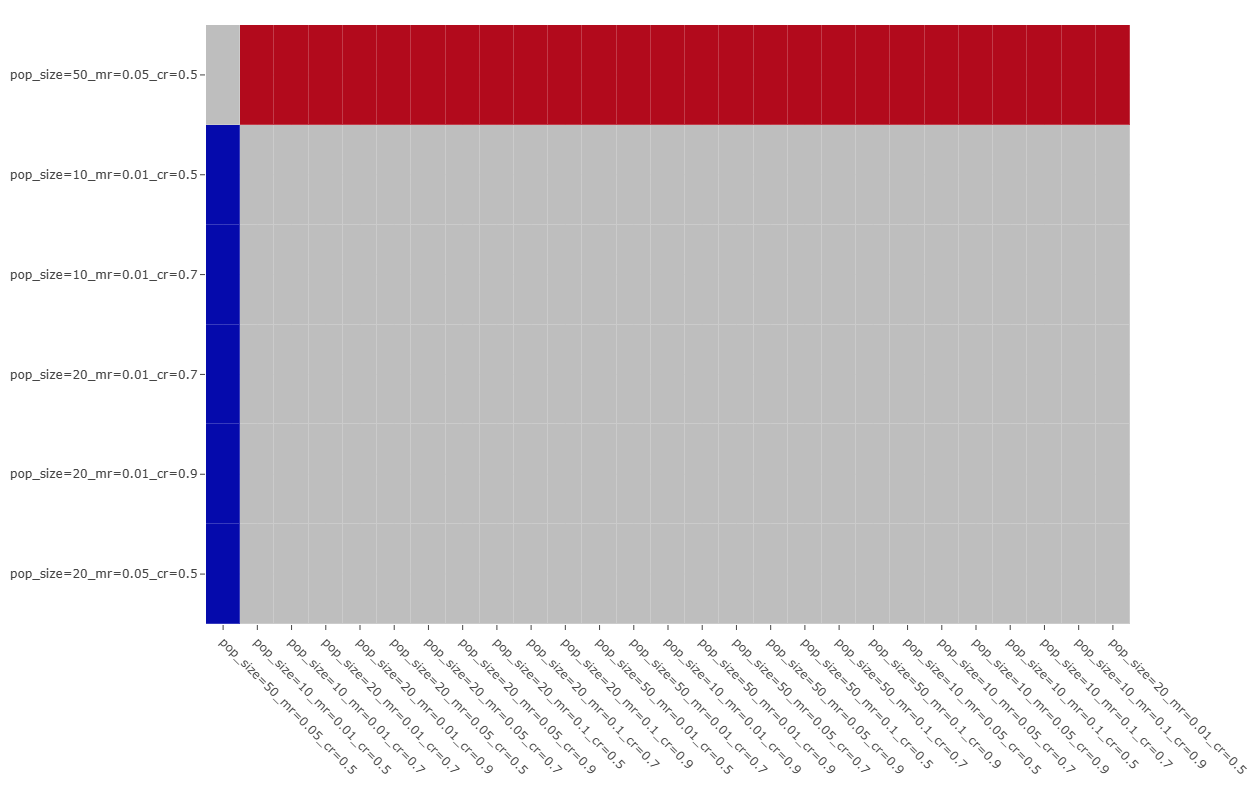
\includegraphics[width=1\linewidth]{Graphs/Katsuura/Ranking.png}
    \caption{Ranking of the function settings. The heatmap generated produces different rankings for each setting, which are marked in blue and red. The optimal settings are ordered and marked in blue, while the least optimal settings are marked in red. The optimal setting is ranked the first, followed by other settings of lower population sizes.}
    \label{fig:ranking-Katsuura}
\end{figure}
Figure \ref{fig:shapley-katsuura} refers to the contribution of each setting to the portfolio. The spacing is taken as linear, and the permutation size of the groups and the functions are set to 3 and 20 respectively. This allows for a more accurate reading, as a lower permutation size for grouping is more accurate, while a higher permutation size for the functions allows to consider higher number of portfolios.  
\begin{figure}[h!]
    \centering
    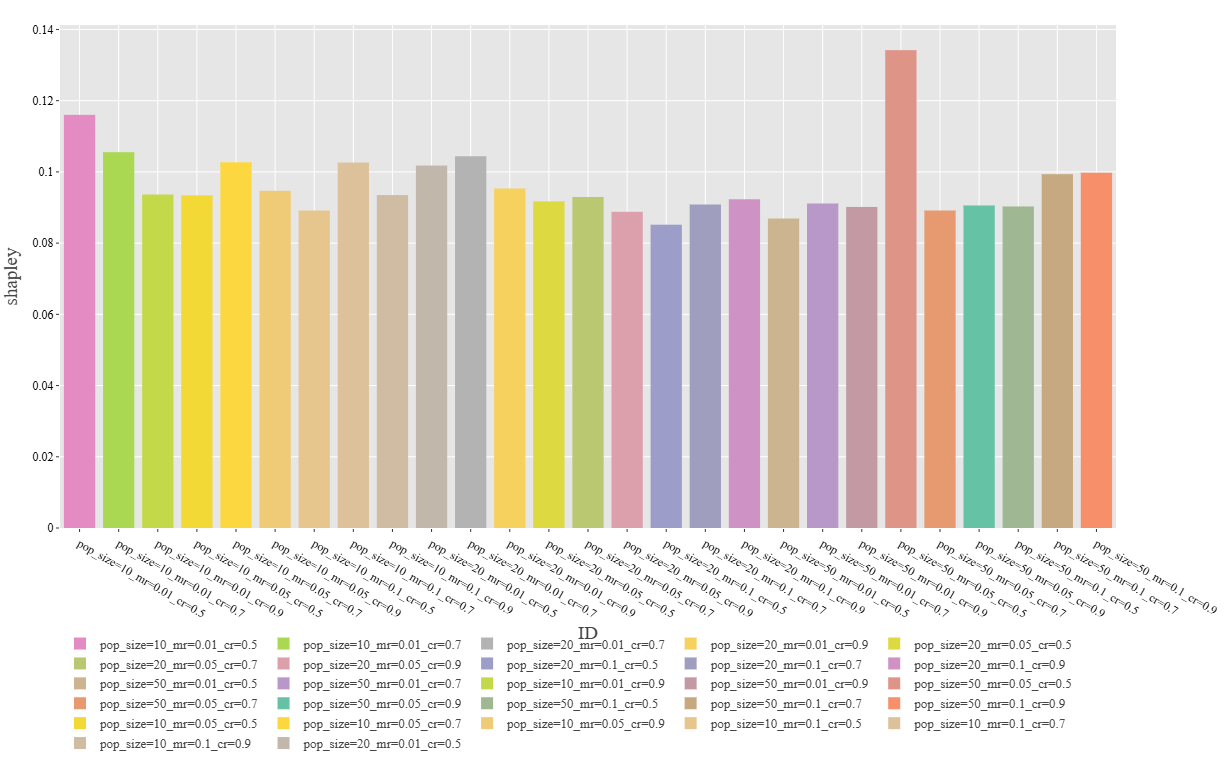
\includegraphics[width=1\linewidth]{Graphs/Katsuura/Shapley_Values.png}
    \caption{Contribution of each setting to the portfolio. The x-axis refers to the function setting, while the y-axis refers to the shape/size of contribution. }
    \label{fig:shapley-katsuura}
\end{figure}



\section{Discussion and Conclusion}\label{sec:dis&res}

%Summarize the results and conclude your report. If you would like to put the main conclusions discussions as lists in this part, you can see an example below.

% \begin{enumerate}[1)]
%     \item We suggest using population size $\mu=x$ for the genetic algorithm to solve the problem.
    
%     \item The genetic algorithm benefits from small mutation rates in solving the \textsc{NAS} problem. (Just an example, this may not be the truth.)
    
%     \item We observe that the evolution strategy benefits from comma selection for solving the \textsc{NAS} problem. (Again, just an example).
% \end{enumerate}
 
 \textbf{Tips:} Please put the references in the file \emph{references.bib} and cite them in the right line, like this \cite{hadash2018estimate}.


\clearpage
\bibliographystyle{unsrt}  
\bibliography{references}  


\end{document}
